\cleardoublepage
\chapter{Parametric study of HIFI's standing waves}
\chaptermark{Parametric study}

%=============================================================================
\section{Model used to explore the parameters}
In this part, I use HIFI as an example.
My goal is to show where each standing wave in HIFI is born.

\begin{figure}[hbtp]
    \centering
    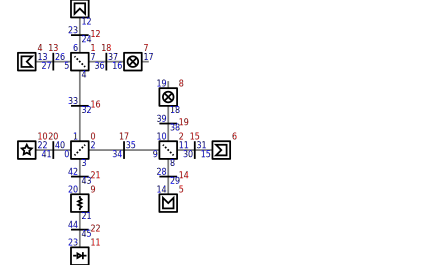
\includegraphics{ports_diplexerband}
    \label{fig:ports_diplexerband}
\end{figure}



%=============================================================================
\section{Folding and calibration}

We are going to assume that the intrinsic sideband ratio of the mixer is 0.5, that is that the mixer is perfectly balanced.  This is of course not the case, but our goal here is to explore the effect of the standing waves on the coupling, not the imperfections of the mixer.

%=============================================================================
\section{Exploration}

At first, the whole system will be as perfect as I can make it.  I do not have a model for a perfect grid, but I can make the grid so thin and dense that it will drown the effect of the grid within the thickness of the line in the plots.

Then, little by little I will make the elements more realistic, and describe the results.

Each time, I present a plot of
\begin{itemize}
    \item the coupling of the mixers to the LO before mixing,
    \item the coupling of the mixers to the sky before mixing,
    \item the coupling of the mixers to the LO after mixing,
    \item the coupling of the mixers to the sky after mixing,
    \item the sideband ratio of the LO.
    \item the sideband ration of the sky.
\end{itemize}

Why do the LO coupling matters?
Because the LO is a source of noise.
And a strong one, think \SI{120}{\kelvin}.
Of course, diplexer bands and beam splitter bands try to minimize the LO coupling, but even \SI{1}{\percent} of \si{120}{\kelvin} matters, remember that the CMB is at \SI{3}{\kelvin}.
Note that this value must be divided by 2: it radiates \SI{120}{\kelvin}, but only half of it goes through the H or V grid, therefore it shines at \SI{60}{\kelvin} in each.

%-----------------------------------------------------------------------------
\clearpage
\subsection{Perfect instrument}
Even in the perfect case, the diplexer is optimally tuned to the center of the IF, and there is a twenty-percent degradation of the coupling at the borders of the IF.

Show that there is a slight offset of the perfect diplexer tuning due to the entry grid not being perfect.

This means that we are correct in taking calibration measures in order to tune the diplexer instead of relying on the value given by the formula.

\begin{figure}[hbtp]
    \centering
    \begin{subfigure}[b]{.5\textwidth}
        \includegraphics{chapter_3/0_ideal_h_dsb}%
        \caption{H mixer power coupling.}
    \end{subfigure}%
    \begin{subfigure}[b]{.5\textwidth}
        \includegraphics{chapter_3/0_ideal_v_dsb}%
        \caption{V mixer power coupling.}
    \end{subfigure}%
    \\
    \begin{subfigure}[b]{.5\textwidth}
        \includegraphics{chapter_3/0_ideal_h_sbr}%
        \caption{H mixer sideband ratio.}
    \end{subfigure}%
    \begin{subfigure}[b]{.5\textwidth}
        \includegraphics{chapter_3/0_ideal_v_sbr}%
        \caption{V mixer sideband ratio.}
    \end{subfigure}%
    \\
    \begin{subfigure}[b]{.5\textwidth}
        \includegraphics{chapter_3/0_ideal_h_ssb}%
        \caption{H mixer folded coupling.}
    \end{subfigure}%
    \begin{subfigure}[b]{.5\textwidth}
        \includegraphics{chapter_3/0_ideal_v_ssb}%
        \caption{V mixer folded coupling.}
    \end{subfigure}%
    \caption{Coupling and sideband ratios of the H and V mixers for an ideal instrument.}
    \label{fig:0_ideal}
\end{figure}

%-----------------------------------------------------------------------------
\clearpage
\subsection{Realistic diplexer grids}

\begin{figure}[hbtp]
    \centering
    \begin{subfigure}[b]{.5\textwidth}
        \includegraphics{chapter_3/02_realgrids_h_dsb}%
        \caption{H mixer power coupling.}
    \end{subfigure}%
    \begin{subfigure}[b]{.5\textwidth}
        \includegraphics{chapter_3/02_realgrids_v_dsb}%
        \caption{V mixer power coupling.}
    \end{subfigure}%
    \\
    \begin{subfigure}[b]{.5\textwidth}
        \includegraphics{chapter_3/02_realgrids_h_sbr}%
        \caption{H mixer sideband ratio.}
    \end{subfigure}%
    \begin{subfigure}[b]{.5\textwidth}
        \includegraphics{chapter_3/02_realgrids_v_sbr}%
        \caption{V mixer sideband ratio.}
    \end{subfigure}%
    \\
    \begin{subfigure}[b]{.5\textwidth}
        \includegraphics{chapter_3/02_realgrids_h_ssb}%
        \caption{H mixer folded coupling.}
    \end{subfigure}%
    \begin{subfigure}[b]{.5\textwidth}
        \includegraphics{chapter_3/02_realgrids_v_ssb}%
        \caption{V mixer folded coupling.}
    \end{subfigure}%
    \caption{Coupling and sideband ratios of the H and V mixers for an ideal instrument.}
    \label{fig:02_realgrids}
\end{figure}

%-----------------------------------------------------------------------------
\clearpage
\subsection{Reflective mixer}
This simulates a desired behavior of the horn: the crosspol must not couple to the mixer.
Well, it would be nice if the crosspol would just disappear, but it is not how rectangular horns work, they reflect what they don't want.

\begin{figure}[hbtp]
    \centering
    \begin{subfigure}[b]{.5\textwidth}
        \includegraphics{chapter_3/03_mh_cr_h_dsb}%
        \caption{H mixer power coupling.}
    \end{subfigure}%
%    \begin{subfigure}[b]{.5\textwidth}
%        \includegraphics{chapter_3/03_mh_cr_v_dsb}%
%        \caption{V mixer power coupling.}
%    \end{subfigure}%
    \\
    \begin{subfigure}[b]{.5\textwidth}
        \includegraphics{chapter_3/03_mh_cr_h_sbr}%
        \caption{H mixer sideband ratio.}
    \end{subfigure}%
%    \begin{subfigure}[b]{.5\textwidth}
%        \includegraphics{chapter_3/03_mh_cr_v_sbr}%
%        \caption{V mixer sideband ratio.}
%    \end{subfigure}%
    \\
    \begin{subfigure}[b]{.5\textwidth}
        \includegraphics{chapter_3/03_mh_cr_h_ssb}%
        \caption{H mixer folded coupling.}
    \end{subfigure}%
%    \begin{subfigure}[b]{.5\textwidth}
%        \includegraphics{chapter_3/03_mh_cr_v_ssb}%
%        \caption{V mixer folded coupling.}
%    \end{subfigure}%
    \caption{H mixer is cross-pol reflective.}
    \label{fig:03_mh_cr}
\end{figure}

Turning on the co-pol reflectivity of the mixer simulates the imperfection of the horn.
\begin{figure}[hbtp]
    \centering
    \begin{subfigure}[b]{.5\textwidth}
        \includegraphics{chapter_3/04_mh_co_h_dsb}%
        \caption{H mixer power coupling.}
    \end{subfigure}%
%    \begin{subfigure}[b]{.5\textwidth}
%        \includegraphics{chapter_3/04_mh_co_v_dsb}%
%        \caption{V mixer power coupling.}
%    \end{subfigure}%
    \\
    \begin{subfigure}[b]{.5\textwidth}
        \includegraphics{chapter_3/04_mh_co_h_sbr}%
        \caption{H mixer sideband ratio.}
    \end{subfigure}%
%    \begin{subfigure}[b]{.5\textwidth}
%        \includegraphics{chapter_3/04_mh_co_v_sbr}%
%        \caption{V mixer sideband ratio.}
%    \end{subfigure}%
    \\
    \begin{subfigure}[b]{.5\textwidth}
        \includegraphics{chapter_3/04_mh_co_h_ssb}%
        \caption{H mixer folded coupling.}
    \end{subfigure}%
%    \begin{subfigure}[b]{.5\textwidth}
%        \includegraphics{chapter_3/04_mh_co_v_ssb}%
%        \caption{V mixer folded coupling.}
%    \end{subfigure}%
    \caption{H mixer is co-pol reflective.}
    \label{fig:04_mh_co}
\end{figure}

Both effects together.
\begin{figure}[hbtp]
    \centering
    \begin{subfigure}[b]{.5\textwidth}
        \includegraphics{chapter_3/05_mh_cocr_h_dsb}%
        \caption{H mixer power coupling.}
    \end{subfigure}%
%    \begin{subfigure}[b]{.5\textwidth}
%        \includegraphics{chapter_3/05_mh_cocr_v_dsb}%
%        \caption{V mixer power coupling.}
%    \end{subfigure}%
    \\
    \begin{subfigure}[b]{.5\textwidth}
        \includegraphics{chapter_3/05_mh_cocr_h_sbr}%
        \caption{H mixer sideband ratio.}
    \end{subfigure}%
%    \begin{subfigure}[b]{.5\textwidth}
%        \includegraphics{chapter_3/05_mh_cocr_v_sbr}%
%        \caption{V mixer sideband ratio.}
%    \end{subfigure}%
    \\
    \begin{subfigure}[b]{.5\textwidth}
        \includegraphics{chapter_3/05_mh_cocr_h_ssb}%
        \caption{H mixer folded coupling.}
    \end{subfigure}%
%    \begin{subfigure}[b]{.5\textwidth}
%        \includegraphics{chapter_3/05_mh_cocr_v_ssb}%
%        \caption{V mixer folded coupling.}
%    \end{subfigure}%
    \caption{H mixer is co-pol and cross-pol reflective.}
    \label{fig:05_mh_cocr}
\end{figure}

As soon as one reflection is turned on, we observe a standing wave pattern.
This is a priori paradoxical.
Indeed, for standing waves to appear, a cavity must exist, that means we need two reflective surfaces and we have only one.

We show that the mixer is actually looking at itself through the leaky grid of the diplexer unit.

%-----------------------------------------------------------------------------
\clearpage
\subsection{Blaming the grids}
We make the grid much thinner and denser, and the standing wave patters from the previous subsection disappears.

\begin{figure}[hbtp]
    \centering
    \begin{subfigure}[b]{.5\textwidth}
        \includegraphics{chapter_3/06_tighter_h_dsb}%
        \caption{H mixer power coupling.}
    \end{subfigure}%
%    \begin{subfigure}[b]{.5\textwidth}
%        \includegraphics{chapter_3/06_tighter_v_dsb}%
%        \caption{V mixer power coupling.}
%    \end{subfigure}%
    \\
    \begin{subfigure}[b]{.5\textwidth}
        \includegraphics{chapter_3/06_tighter_h_sbr}%
        \caption{H mixer sideband ratio.}
    \end{subfigure}%
%    \begin{subfigure}[b]{.5\textwidth}
%        \includegraphics{chapter_3/06_tighter_v_sbr}%
%        \caption{V mixer sideband ratio.}
%    \end{subfigure}%
    \\
    \begin{subfigure}[b]{.5\textwidth}
        \includegraphics{chapter_3/06_tighter_h_ssb}%
        \caption{H mixer folded coupling.}
    \end{subfigure}%
%    \begin{subfigure}[b]{.5\textwidth}
%        \includegraphics{chapter_3/06_tighter_v_ssb}%
%        \caption{V mixer folded coupling.}
%    \end{subfigure}%
    \caption{Tighter grids.}
    \label{fig:06_tighter}
\end{figure}

We make the grid coarser and it gets worse.

\begin{figure}[hbtp]
    \centering
    \begin{subfigure}[b]{.5\textwidth}
        \includegraphics{chapter_3/07_looser_h_dsb}%
        \caption{H mixer power coupling.}
    \end{subfigure}%
%    \begin{subfigure}[b]{.5\textwidth}
%        \includegraphics{chapter_3/07_looser_v_dsb}%
%        \caption{V mixer power coupling.}
%    \end{subfigure}%
    \\
    \begin{subfigure}[b]{.5\textwidth}
        \includegraphics{chapter_3/07_looser_h_sbr}%
        \caption{H mixer sideband ratio.}
    \end{subfigure}%
%    \begin{subfigure}[b]{.5\textwidth}
%        \includegraphics{chapter_3/07_looser_v_sbr}%
%        \caption{V mixer sideband ratio.}
%    \end{subfigure}%
    \\
    \begin{subfigure}[b]{.5\textwidth}
        \includegraphics{chapter_3/07_looser_h_ssb}%
        \caption{H mixer folded coupling.}
    \end{subfigure}%
%    \begin{subfigure}[b]{.5\textwidth}
%        \includegraphics{chapter_3/07_looser_v_ssb}%
%        \caption{V mixer folded coupling.}
%    \end{subfigure}%
    \caption{Looser grids.}
    \label{fig:07_looser}
\end{figure}

There is a limit on how coarse you can make the grid, as the grid model my Houde makes assumptions on the radius of the wires, their spacing, and the wavelength.

With insanely bad grids, we show that the standing wave pattern is actually far from sinusoidal, as the cavity has a very high Q.

%-----------------------------------------------------------------------------
\clearpage
\subsection{Imperfect rooftop mirrors}
This is how we can achieve the first exchange of polarization power.
Indeed, if we make only the co-pol of the mixer reflective, with an imperfect roof-top mirror we observe standing wave patters on the two polarizations.

\begin{figure}[hbtp]
    \centering
    \begin{subfigure}[b]{.5\textwidth}
        \includegraphics{chapter_3/08_badrt_mhcr_h_dsb}%
        \caption{H mixer power coupling.}
    \end{subfigure}%
%    \begin{subfigure}[b]{.5\textwidth}
%        \includegraphics{chapter_3/08_badrt_mhcr_v_dsb}%
%        \caption{V mixer power coupling.}
%    \end{subfigure}%
    \\
    \begin{subfigure}[b]{.5\textwidth}
        \includegraphics{chapter_3/08_badrt_mhcr_h_sbr}%
        \caption{H mixer sideband ratio.}
    \end{subfigure}%
%    \begin{subfigure}[b]{.5\textwidth}
%        \includegraphics{chapter_3/08_badrt_mhcr_v_sbr}%
%        \caption{V mixer sideband ratio.}
%    \end{subfigure}%
    \\
    \begin{subfigure}[b]{.5\textwidth}
        \includegraphics{chapter_3/08_badrt_mhcr_h_ssb}%
        \caption{H mixer folded coupling.}
    \end{subfigure}%
%    \begin{subfigure}[b]{.5\textwidth}
%        \includegraphics{chapter_3/08_badrt_mhcr_v_ssb}%
%        \caption{V mixer folded coupling.}
%    \end{subfigure}%
    \caption{Imperfect rooftop mirror, mixer cross-reflective.}
    \label{fig:08_badrt_mhcr}
\end{figure}

\begin{figure}[hbtp]
    \centering
    \begin{subfigure}[b]{.5\textwidth}
        \includegraphics{chapter_3/09_badrt_mhcrco_h_dsb}%
        \caption{H mixer power coupling.}
    \end{subfigure}%
%    \begin{subfigure}[b]{.5\textwidth}
%        \includegraphics{chapter_3/09_badrt_mhcrco_v_dsb}%
%        \caption{V mixer power coupling.}
%    \end{subfigure}%
    \\
    \begin{subfigure}[b]{.5\textwidth}
        \includegraphics{chapter_3/09_badrt_mhcrco_h_sbr}%
        \caption{H mixer sideband ratio.}
    \end{subfigure}%
%    \begin{subfigure}[b]{.5\textwidth}
%        \includegraphics{chapter_3/09_badrt_mhcrco_v_sbr}%
%        \caption{V mixer sideband ratio.}
%    \end{subfigure}%
    \\
    \begin{subfigure}[b]{.5\textwidth}
        \includegraphics{chapter_3/09_badrt_mhcrco_h_ssb}%
        \caption{H mixer folded coupling.}
    \end{subfigure}%
%    \begin{subfigure}[b]{.5\textwidth}
%        \includegraphics{chapter_3/09_badrt_mhcrco_v_ssb}%
%        \caption{V mixer folded coupling.}
%    \end{subfigure}%
    \caption{Imperfect rooftop mirror, mixer cross- and co-reflective.}
    \label{fig:09_badrt_mhcrco}
\end{figure}

We can also observe a beat of the standing wave patterns.  This is due to the two arms of the diplexer units being of different length.  A fourrier transform can reveal two picks.
In fact, every cavity involving the diplexer will show these picks.

%-----------------------------------------------------------------------------
\clearpage
\subsection{Mixer phase factor}
\begin{figure}[hbtp]
    \centering
    \begin{subfigure}[b]{.5\textwidth}
        \includegraphics{chapter_3/09_badrt_mhcrco_h_dsb}%
        \caption{DSB, phase \SI{180}{\degree}.}
    \end{subfigure}%
    \begin{subfigure}[b]{.5\textwidth}
        \includegraphics{chapter_3/09_badrt_mhcrco_h_ssb}%
        \caption{SSB, phase \SI{180}{\degree}.}
    \end{subfigure}%
    \\
    \begin{subfigure}[b]{.5\textwidth}
        \includegraphics{chapter_3/10_phase_a_h_dsb}%
        \caption{DSB, phase \SI{150}{\degree}.}
    \end{subfigure}%
    \begin{subfigure}[b]{.5\textwidth}
        \includegraphics{chapter_3/10_phase_a_h_ssb}%
        \caption{SSB, phase \SI{150}{\degree}.}
    \end{subfigure}%
    \\
    \begin{subfigure}[b]{.5\textwidth}
        \includegraphics{chapter_3/11_phase_b_h_dsb}%
        \caption{DSB, phase \SI{120}{\degree}.}
    \end{subfigure}%
    \begin{subfigure}[b]{.5\textwidth}
        \includegraphics{chapter_3/11_phase_b_h_ssb}%
        \caption{SSB, phase \SI{120}{\degree}.}
    \end{subfigure}%
    \caption{Effect of the mixer reflection phase factor.}
    \label{fig:mixer_phase_factor}
\end{figure}

%-----------------------------------------------------------------------------
\clearpage
\subsection{Turn on the LO reflection}
This creates a very strong modulation on top of all the others.
This also allows the two mixers to see each other.
Indeed, because the entry grid leaks, some standing wave patters in one polarization will affect the other after reflection on the local oscillator.

\begin{figure}[hbtp]
    \centering
    \begin{subfigure}[b]{.5\textwidth}
        \includegraphics{chapter_3/12_lor_att00_h_dsb}%
        \caption{H mixer power coupling.}
    \end{subfigure}%
    \begin{subfigure}[b]{.5\textwidth}
        \includegraphics{chapter_3/12_lor_att00_v_dsb}%
        \caption{V mixer power coupling.}
    \end{subfigure}%
    \\
    \begin{subfigure}[b]{.5\textwidth}
        \includegraphics{chapter_3/12_lor_att00_h_sbr}%
        \caption{H mixer sideband ratio.}
    \end{subfigure}%
    \begin{subfigure}[b]{.5\textwidth}
        \includegraphics{chapter_3/12_lor_att00_v_sbr}%
        \caption{V mixer sideband ratio.}
    \end{subfigure}%
    \\
    \begin{subfigure}[b]{.5\textwidth}
        \includegraphics{chapter_3/12_lor_att00_h_ssb}%
        \caption{H mixer folded coupling.}
    \end{subfigure}%
    \begin{subfigure}[b]{.5\textwidth}
        \includegraphics{chapter_3/12_lor_att00_v_ssb}%
        \caption{V mixer folded coupling.}
    \end{subfigure}%
    \caption{LO reflection turned on.}
    \label{fig:12_lor_att00}
\end{figure}

%-----------------------------------------------------------------------------
\clearpage
\subsection{Effect of the attenuator in front of the local oscillator}
Reduces the cross talk and the LO standing waves.

\begin{figure}[hbtp]
    \centering
    \begin{subfigure}[b]{.5\textwidth}
        \includegraphics{chapter_3/13_lor_att10_h_dsb}%
        \caption{H mixer power coupling.}
    \end{subfigure}%
    \begin{subfigure}[b]{.5\textwidth}
        \includegraphics{chapter_3/13_lor_att10_v_dsb}%
        \caption{V mixer power coupling.}
    \end{subfigure}%
    \\
    \begin{subfigure}[b]{.5\textwidth}
        \includegraphics{chapter_3/13_lor_att10_h_sbr}%
        \caption{H mixer sideband ratio.}
    \end{subfigure}%
    \begin{subfigure}[b]{.5\textwidth}
        \includegraphics{chapter_3/13_lor_att10_v_sbr}%
        \caption{V mixer sideband ratio.}
    \end{subfigure}%
    \\
    \begin{subfigure}[b]{.5\textwidth}
        \includegraphics{chapter_3/13_lor_att10_h_ssb}%
        \caption{H mixer folded coupling.}
    \end{subfigure}%
    \begin{subfigure}[b]{.5\textwidth}
        \includegraphics{chapter_3/13_lor_att10_v_ssb}%
        \caption{V mixer folded coupling.}
    \end{subfigure}%
    \caption{LO reflection turned on, \SI{10}{\decibel} attenuator.}
    \label{fig:13_lor_att10}
\end{figure}

%-----------------------------------------------------------------------------
\clearpage
\subsection{Reflective source}
Looking at the hot black body.
\begin{figure}[hbtp]
    \centering
    \begin{subfigure}[b]{.5\textwidth}
        \includegraphics{chapter_3/14_hbb_h_dsb}%
        \caption{H mixer power coupling.}
    \end{subfigure}%
    \begin{subfigure}[b]{.5\textwidth}
        \includegraphics{chapter_3/14_hbb_v_dsb}%
        \caption{V mixer power coupling.}
    \end{subfigure}%
    \\
    \begin{subfigure}[b]{.5\textwidth}
        \includegraphics{chapter_3/14_hbb_h_sbr}%
        \caption{H mixer sideband ratio.}
    \end{subfigure}%
    \begin{subfigure}[b]{.5\textwidth}
        \includegraphics{chapter_3/14_hbb_v_sbr}%
        \caption{V mixer sideband ratio.}
    \end{subfigure}%
    \\
    \begin{subfigure}[b]{.5\textwidth}
        \includegraphics{chapter_3/14_hbb_h_ssb}%
        \caption{H mixer folded coupling.}
    \end{subfigure}%
    \begin{subfigure}[b]{.5\textwidth}
        \includegraphics{chapter_3/14_hbb_v_ssb}%
        \caption{V mixer folded coupling.}
    \end{subfigure}%
    \caption{Looking at the hot black body.}
    \label{fig:14_hbb}
\end{figure}

%-----------------------------------------------------------------------------
\clearpage
\subsection{Reflective V mixer}
\begin{figure}[hbtp]
    \centering
    \begin{subfigure}[b]{.5\textwidth}
        \includegraphics{chapter_3/15_everything_h_dsb}%
        \caption{H mixer power coupling.}
    \end{subfigure}%
    \begin{subfigure}[b]{.5\textwidth}
        \includegraphics{chapter_3/15_everything_v_dsb}%
        \caption{V mixer power coupling.}
    \end{subfigure}%
    \\
    \begin{subfigure}[b]{.5\textwidth}
        \includegraphics{chapter_3/15_everything_h_sbr}%
        \caption{H mixer sideband ratio.}
    \end{subfigure}%
    \begin{subfigure}[b]{.5\textwidth}
        \includegraphics{chapter_3/15_everything_v_sbr}%
        \caption{V mixer sideband ratio.}
    \end{subfigure}%
    \\
    \begin{subfigure}[b]{.5\textwidth}
        \includegraphics{chapter_3/15_everything_h_ssb}%
        \caption{H mixer folded coupling.}
    \end{subfigure}%
    \begin{subfigure}[b]{.5\textwidth}
        \includegraphics{chapter_3/15_everything_v_ssb}%
        \caption{V mixer folded coupling.}
    \end{subfigure}%
    \caption{Looking at the hot black body.}
    \label{fig:15_everything}
\end{figure}

\subsection{Simulated diplexer scans}
These reproduce distorsions observed on real diplexer scans.

\subsection{Influence of the diplexer tuning on the cross talk}
Show that mistuning one diplexer has an effect on the coupling of the mixer in the other branch.
